\section{Related Work}

Many authors have worked in the same area~\citep*{leal2015optimizing}. In special,  \citeauthor{espinosa2019reinforcement} have discussed more in detail.

\begin{equation}\label{euler_eq}
    e^{ \pm i\theta } = \cos \theta \pm i\sin \theta
\end{equation}

It is easy to see that Eq.\ref{euler_eq} is the most beautiful equation. You can also cite software like scikit-learn~\citep{scikit-learn} or long urls~\citep{GartnerNFC}.

\kant[3-5]

\begin{figure}
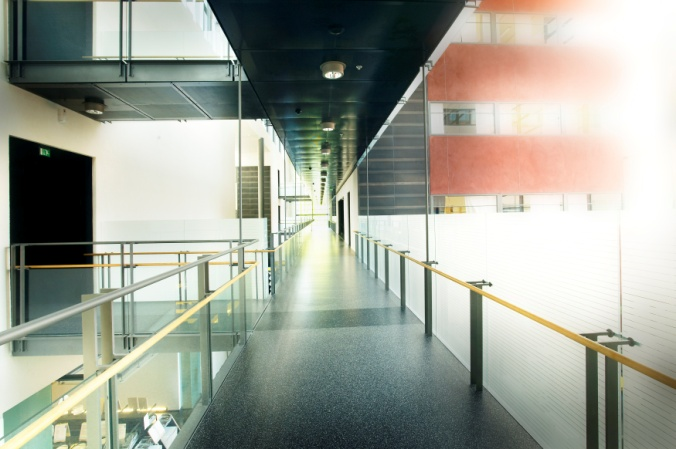
\includegraphics[width=8cm]{figures/arcada.jpg}
\caption{The interior of Arcada. Photograph Valtteri Kantanen Arcada 2008}
\end{figure}

\kant[2]
